\section{Graphen}
Ein Graph ist ein Paar (V, E), wobei:
\begin{itemize}
    \item V ist ein Set von Vertizes (Knoten)
    \item E ist eine Collection von Vertizes-Paaren, Kanten (Edge)
    \item Vertizes und Kanten sind Positionen und speichern Elemente
\end{itemize}

\subsection{Kanten-Typen}
\begin{itemize}
    \item gerichtete Kanten
    \begin{itemize}
        \item geordnetes Paar von Vertizes (u,v)
        \item erster Vertex u entspricht dem Ursprung
        \item zweiter Vertex v entspricht dem Ziel
        \item z.B. Flug
    \end{itemize}
    \item ungerichtete Kanten
    \begin{itemize}
        \item ungeordnetes Vertizes-Paar (u,v)
        \item z.B. Flugroute
    \end{itemize}
    \item gerichteter Graph
    \begin{itemize}
        \item alle Kanten sind gerichtet
        \item z.B. Flugplan
    \end{itemize}
    \item ungerichter Graph
    \begin{itemize}
        \item alle Kanten sind ungerichtet
        \item z.B. Flugrouten-Plan
    \end{itemize}
\end{itemize}


\subsection{Laufzeit}
\begin{center}
    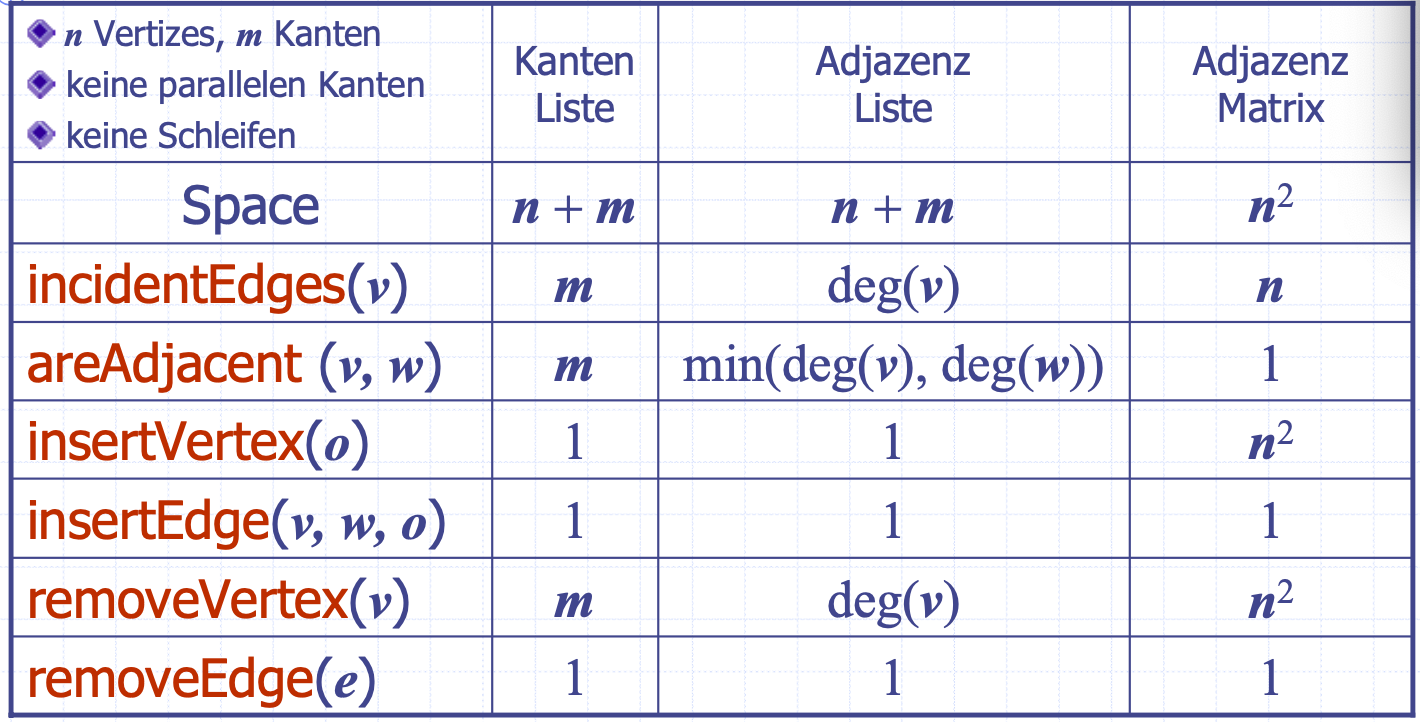
\includegraphics[scale=.2]{graphic/11 Graph/Laufzeit.png}
\end{center}
\vspace{-8pt}


\subsection{Terminologie}
\begin{itemize}
    \item Kanten sind \textbf{inzident} (enden) an einem Vertex
    \item \textbf{Adjazente} (benachbarte) Vertizes
    \item \textbf{Grad (Degree)} eines Vertex: Anzahl inzidenter Kanten
    \item \textbf{Parallele Kanten}
    \item \textbf{Schleife}
    \item \textbf{Pfad}
    \begin{itemize}
        \item Sequenz von alternierenden Vertizes und Kanten
        \item beginnt mit einem Vertex
        \item endet mit einem Vertex
        \item jede Kante beginnt und endet an einem ihrer Endpunkte
    \end{itemize}
    \item \textbf{Einfacher Pfad}
    \begin{itemize}
        \item ein Pfad, so dass alle seine Vertizes und Kanten unterschiedlich sind
    \end{itemize}
    \item \textbf{Zyklus}
    \begin{itemize}
        \item zirkuläre Sequenz alternierender Vertizes und Kanten
    \end{itemize}
    \item \textbf{Einfacher Zyklus}
    \begin{itemize}
        \item ein Zyklus, so dass alle seine Vertizes und Kanten unterschiedlich sind
    \end{itemize}
\end{itemize}


\subsection{Eigenschaften}
\begin{itemize}
    \item \textbf{Notation:}
    \begin{itemize}
        \item n = Anzahl Vertizes
        \item m = Anzahl Kanten
        \item deg(v) = Grad von Vertex v
    \end{itemize}
    \item \textbf{Eigenschaft 1:}
    \begin{itemize}
        \item $\Sigma_v deg(v) = 2m$
        \item Beweis: jede Kante wird zweimal gezählt
    \end{itemize}
    \item \textbf{Eigenschaft 2:}
     \begin{itemize}
        \item In einem ungerichteten Graphen ohne Schleifen und ohne parallele Kanten gilt:
        \item m $\leqslant$  n (n - 1) / 2
        \item entspricht einem ungerichteten, einfachen Graphen
        \item Beweis: jeder Vertex besitzt einen Grad von höchstens (n - 1)
     \end{itemize}
\end{itemize}

\vspace{-8pt}
\begin{center}
    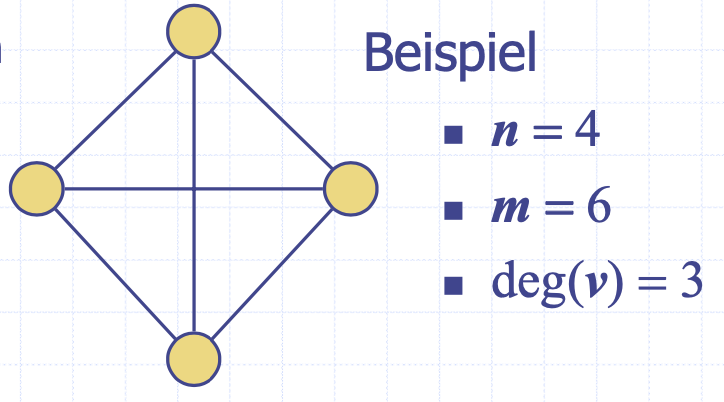
\includegraphics[scale=.25]{graphic/11 Graph/Eigenschaften.png}
\end{center}
\vspace{-8pt}


\subsection{Haupt-Methoden}
\begin{center}
    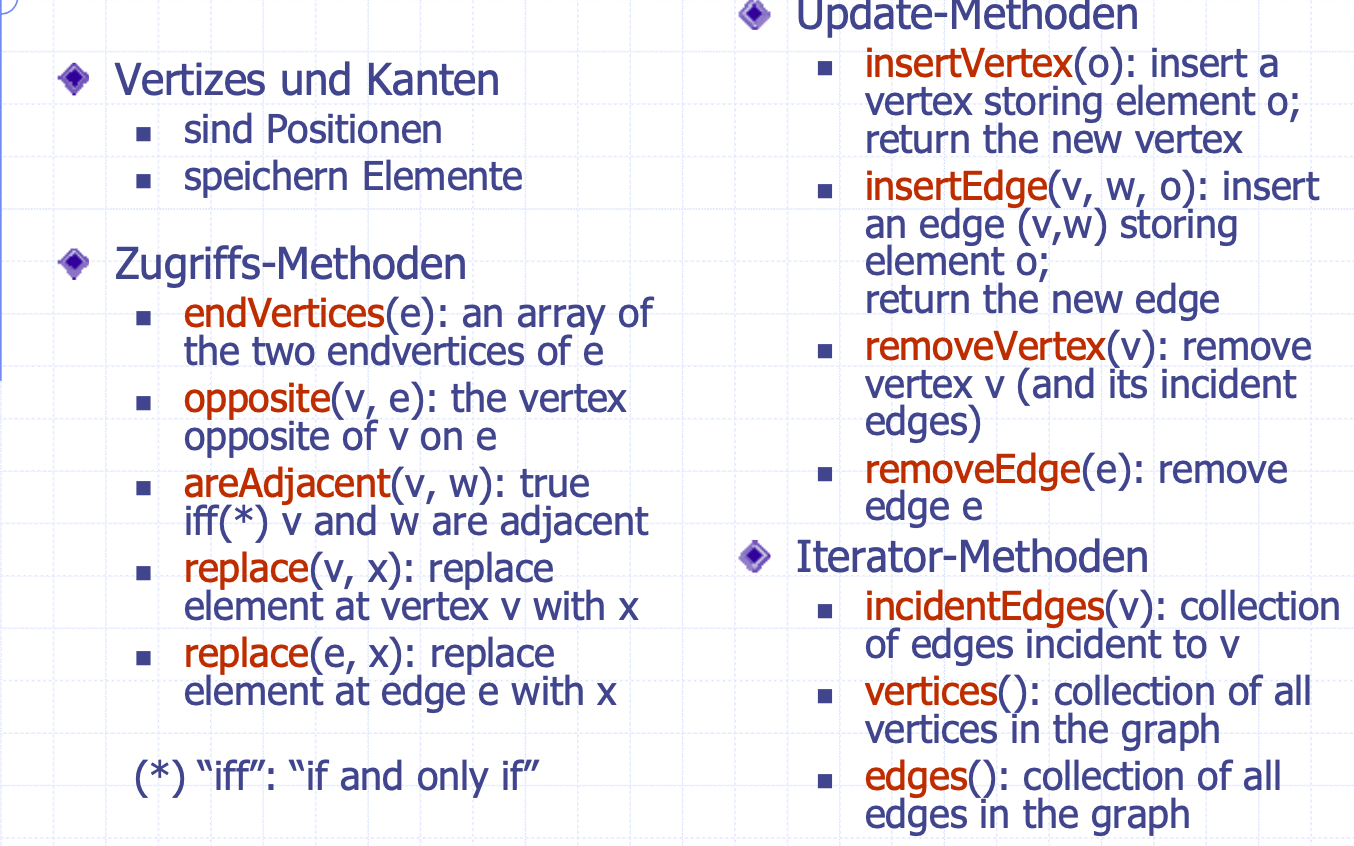
\includegraphics[scale=.25]{graphic/11 Graph/Methoden.png}
\end{center}
\vspace{-8pt}


\subsection{Struktur}

\subsubsection{Kanten-Listen}

\begin{center}
    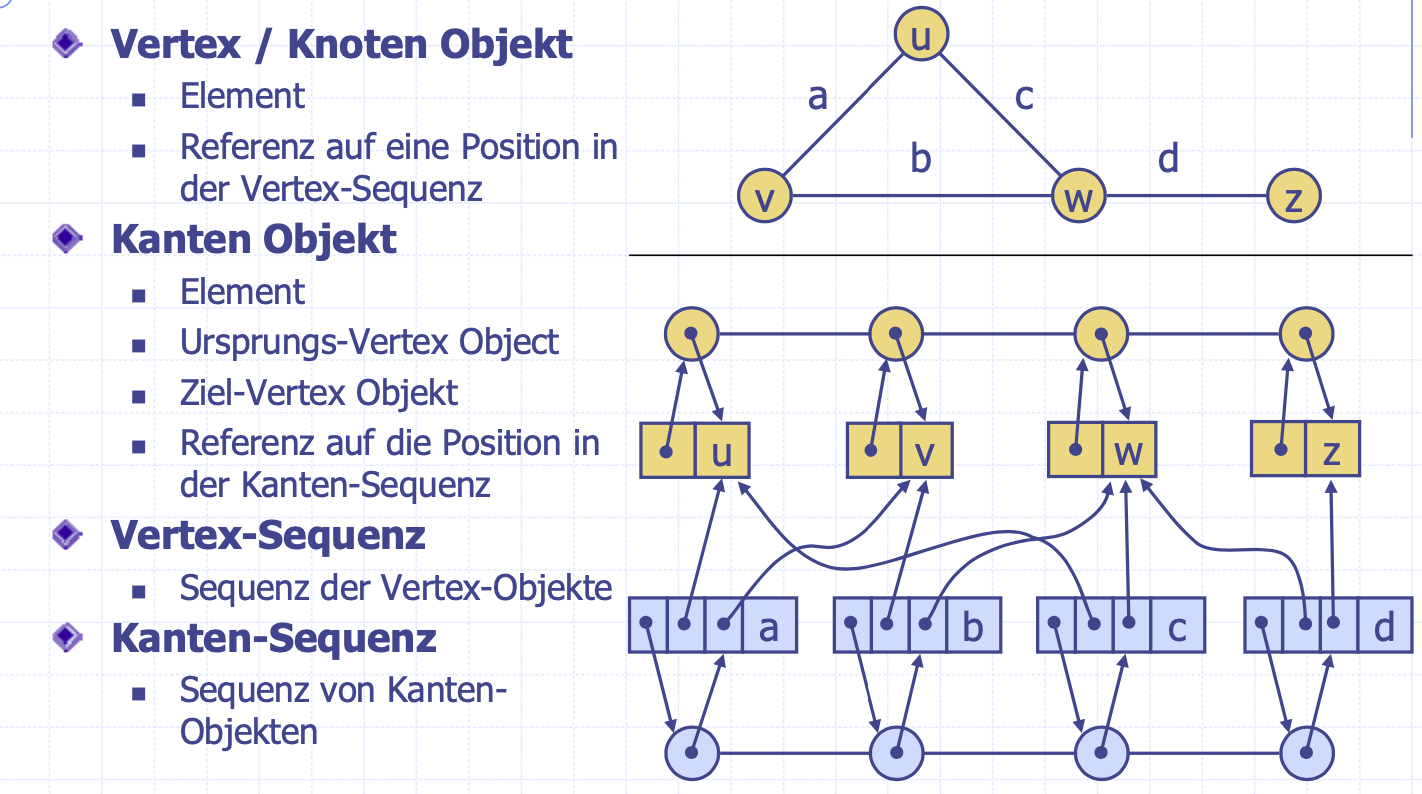
\includegraphics[scale=.23]{graphic/11 Graph/Kanten-Listen.png}
\end{center}
\vspace{-8pt}

\subsubsection{Adjazenz-Listen}
\begin{center}
    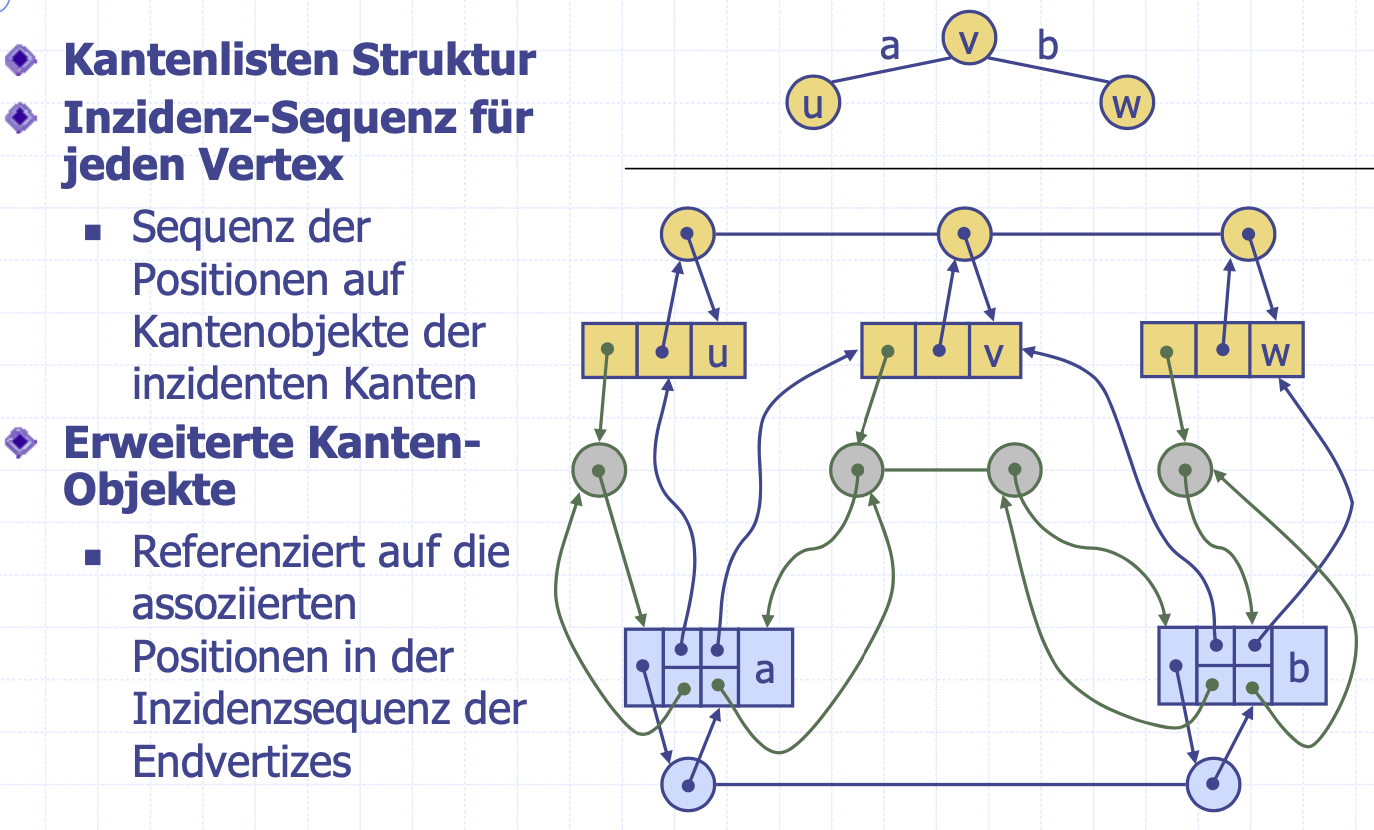
\includegraphics[scale=.23]{graphic/11 Graph/Adjazenz-Listen.png}
\end{center}
\vspace{-8pt}


\subsubsection{Adjazenz-Matrix}
\begin{center}
    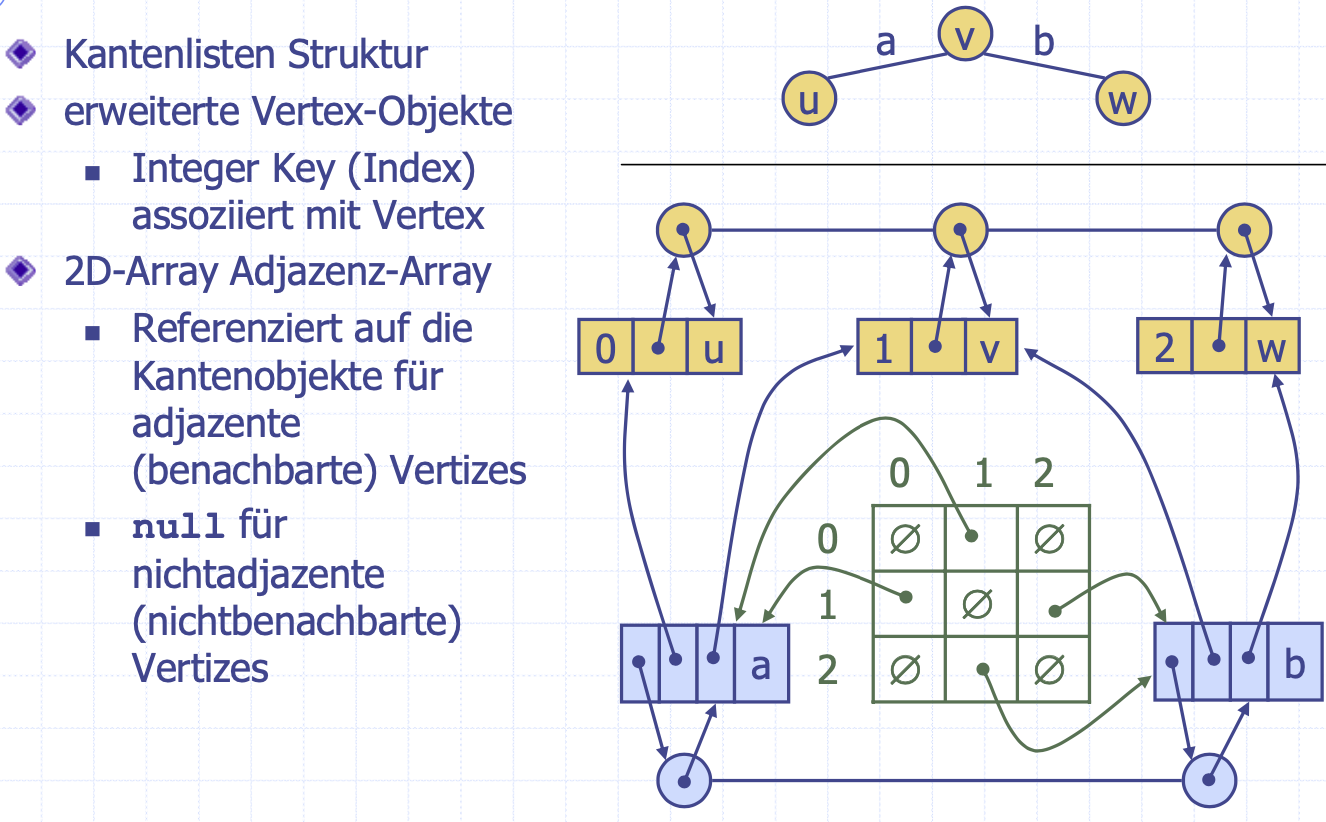
\includegraphics[scale=.23]{graphic/11 Graph/Adjazenz-Matrix.png}
\end{center}
\vspace{-8pt}


\subsection{Subgraphen}
\begin{center}
    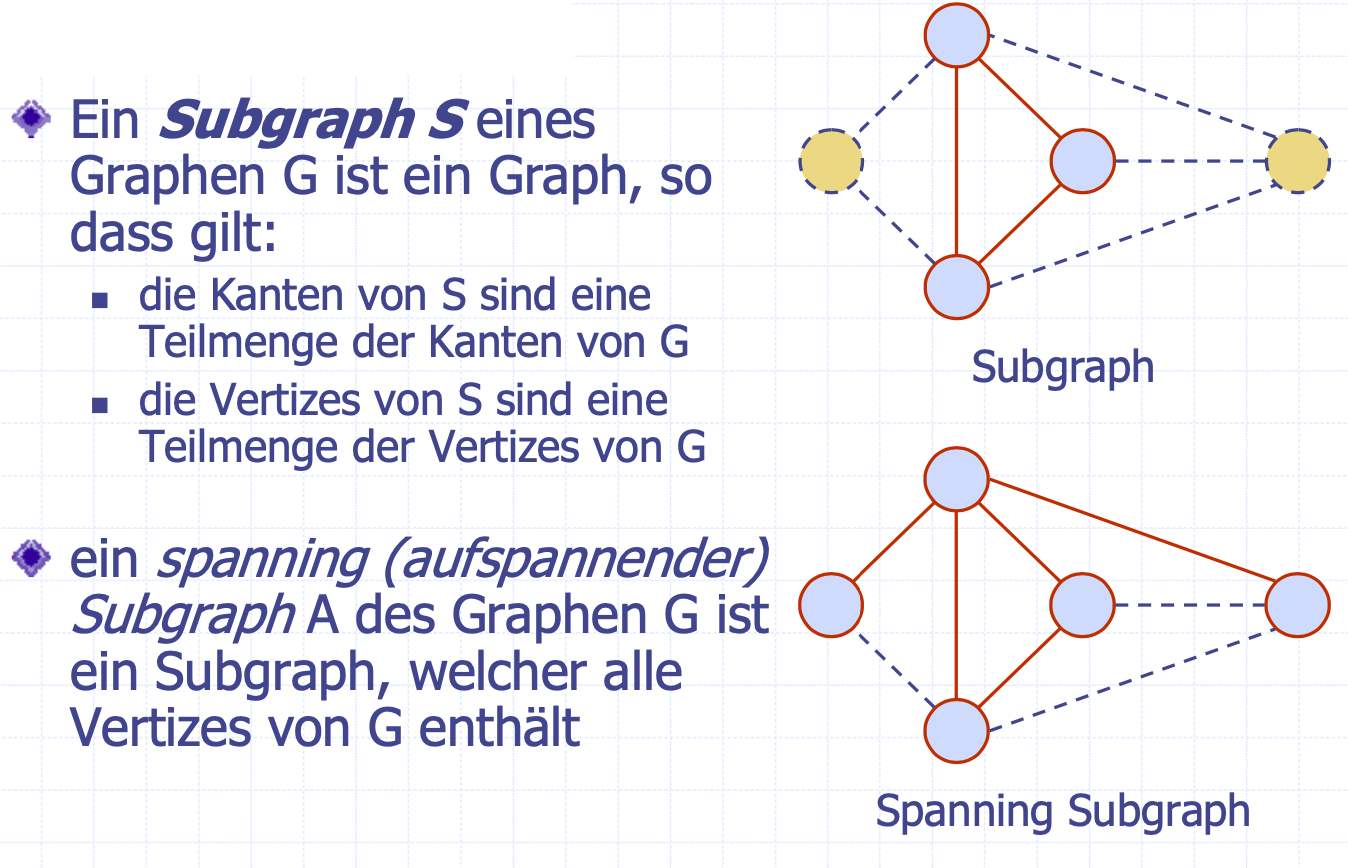
\includegraphics[scale=.23]{graphic/11 Graph/Subgraphen.png}
\end{center}
\vspace{-8pt}

\subsection{Connectivity}
\begin{center}
    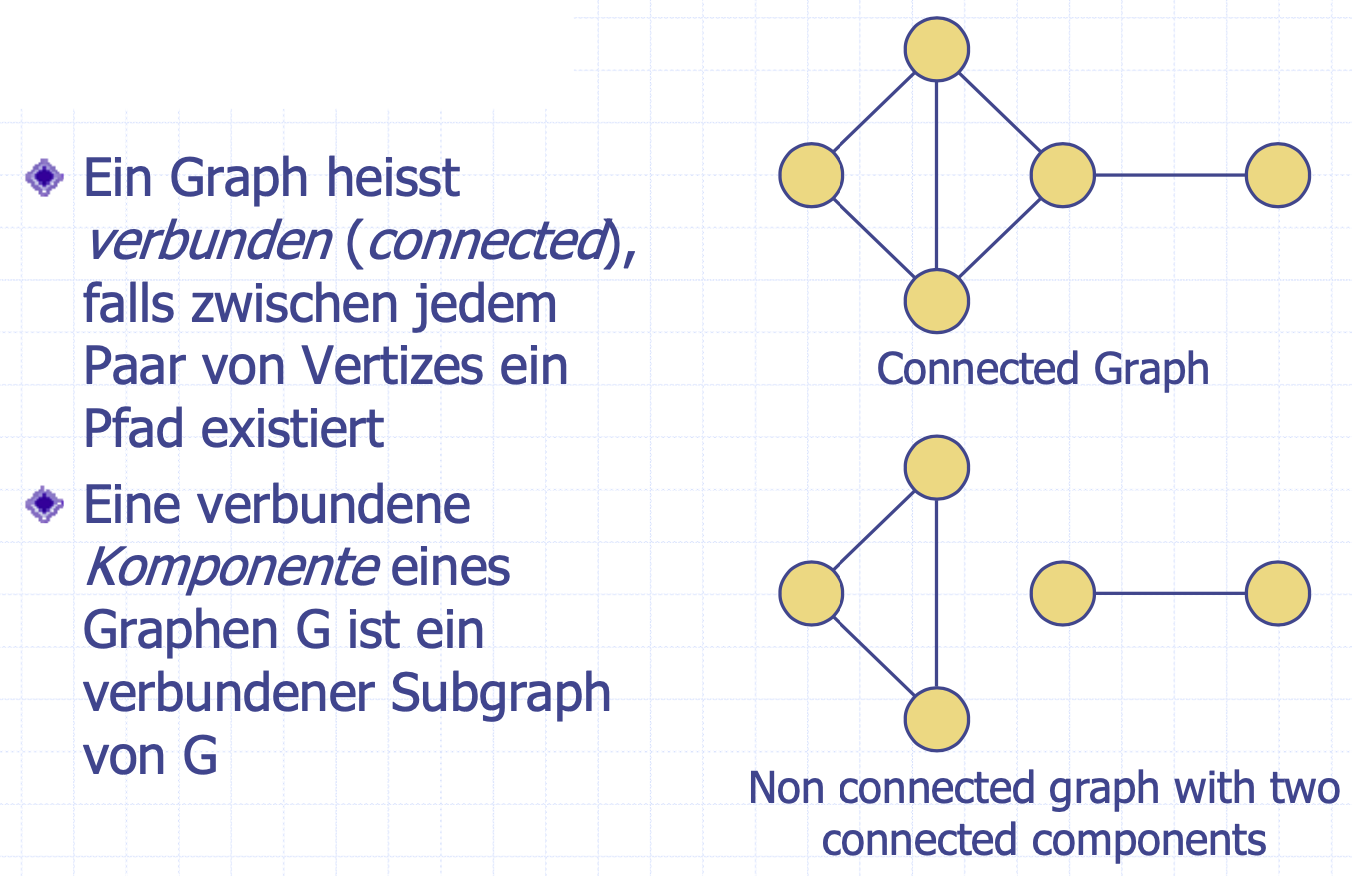
\includegraphics[scale=.2]{graphic/11 Graph/Connectivity.png}
\end{center}
\vspace{-8pt}


\subsection{Bäume und Wälder}
\begin{center}
    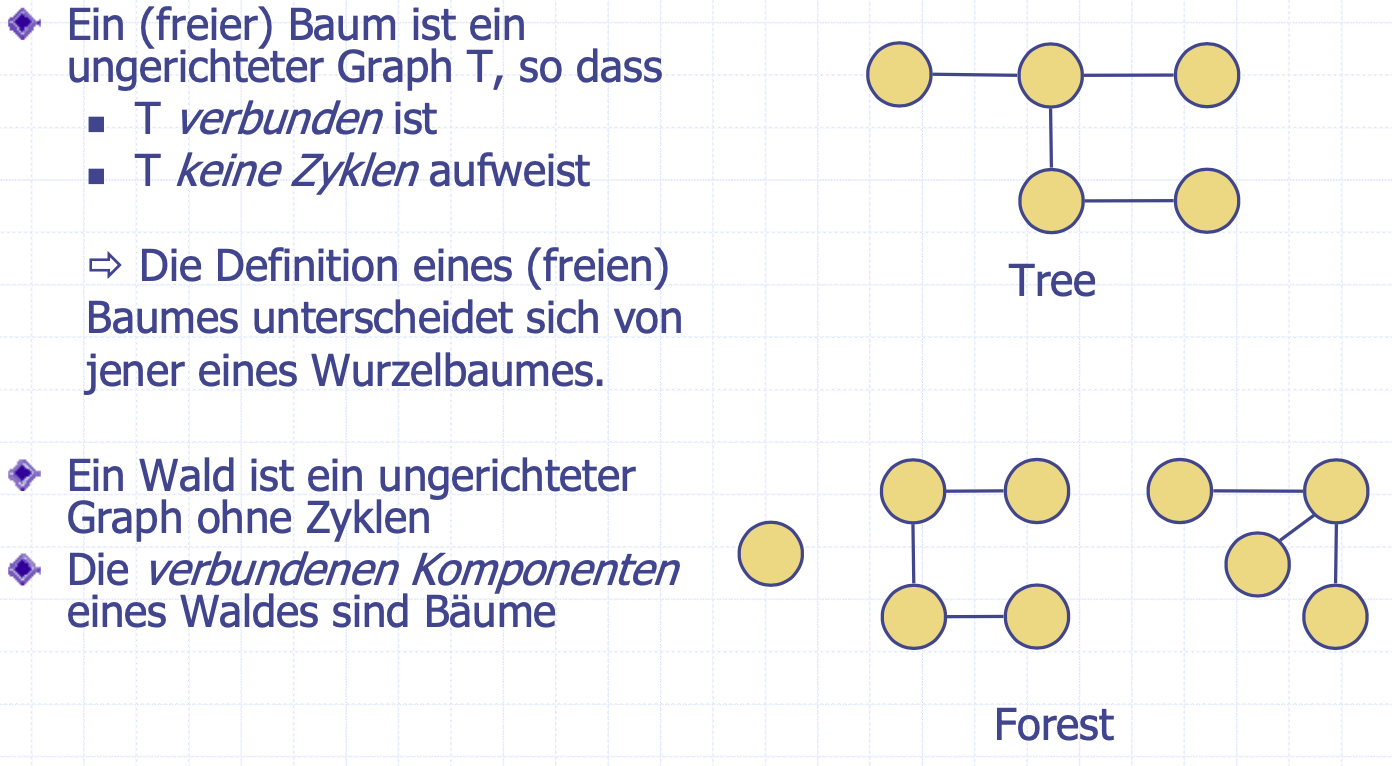
\includegraphics[scale=.23]{graphic/11 Graph/Bäume und Wälder1.png}
\end{center}
\vspace{-8pt}


\subsection{Spanning Trees und Wälder}
\begin{center}
    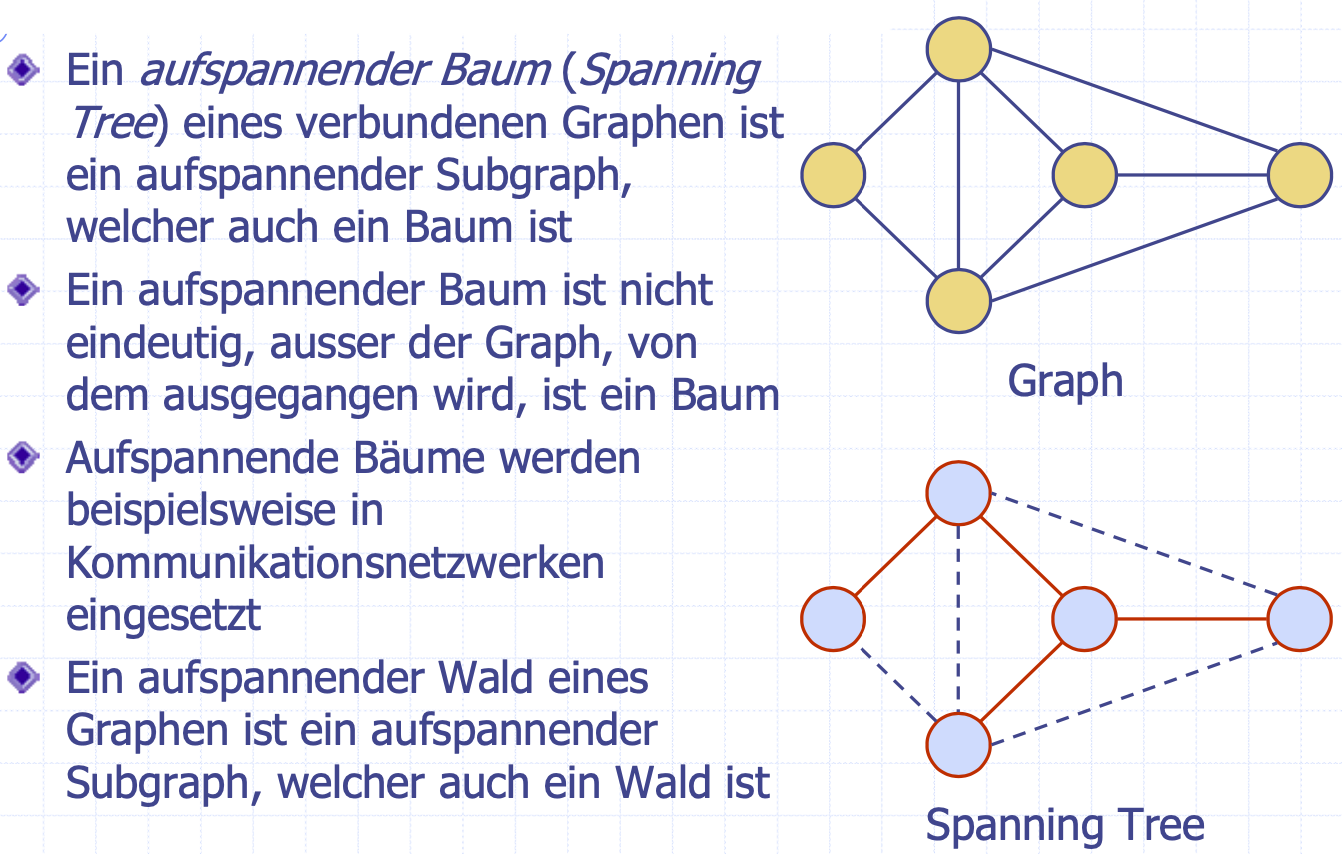
\includegraphics[scale=.25]{graphic/11 Graph/Bäume und Wälder2.png}
\end{center}
\vspace{-8pt}

\vfill
$ $
\columnbreak

\paragraph{Graph Implementation}

\begin{lstlisting}
public class KantenListenGraph {
    private DoubleLinkedPosition<Vertex> vSeqHead;
    private DoubleLinkedPosition<Edge> eSeqHead;
    
    public Vertex insertVertex(Object o) {
        vSeqHead = new DoubleLinkedPosition<Vertex>(vSeqHead);
        Vertex vertex = new Vertex(o, vSeqHead);
        return vertex;
    }
    
    public Edge insertEdge(Vertex v, Vertex w, Object o) {
        Vertex[] endVertices = {v, w};
        eSeqHead = new DoubleLinkedPosition<Edge>(eSeqHead);
        Edge edge = new Edge(o, endVertices, eSeqHead);
        return edge;
    }

public class Vertex {
    private Object object;
    protected DoubleLinkedPosition<Vertex> position;
    
    public Vertex(Object o, DoubleLinkedPosition<Vertex> position) {
        this.object = o;
        this.position = position;
        position.element = this;
  }

public class Edge {
    private Object object;
    private Vertex[] vertices;
    protected DoubleLinkedPosition<Edge> position;
    
    public Edge(Object o, Vertex[] vertices, DoubleLinkedPosition<Edge> position) {
        this.object = o;
        this.vertices = vertices;
        this.position = position;
        position.element = this;
}

public class DoubleLinkedPosition<E> {
    protected DoubleLinkedPosition<E> previous;
    protected DoubleLinkedPosition<E> next;
    protected E element;
    
    DoubleLinkedPosition(DoubleLinkedPosition<E> next) {
        this.next = next;
        if (next != null) {
            next.previous = this;
        }
    }
}
\end{lstlisting}


\newpage